\documentclass[11pt]{article} % For LaTeX2e
\usepackage{palatino}
\usepackage{graphicx}
\usepackage{svg}
\usepackage{amsmath}
\usepackage{soul}
\usepackage{color}
\usepackage{pslatex}
\usepackage{apacite}
\usepackage{float} % Roger Levy added this and changed figure/table
                   % placement to [H] for conformity to Word template,
                   % though floating tables and figures to top is
                   % still generally recommended!
\usepackage{url}

\usepackage[colorinlistoftodos]{todonotes}

% \usepackage{cogsci}

\usepackage{setspace}
\doublespacing

\newcommand{\detailtexcount}[1]{%
  \immediate\write18{texcount -merge -sum -q #1.tex output.bbl > #1.wcdetail }%
  \verbatiminput{#1.wcdetail}%
}

\newcommand{\quickwordcount}[1]{%
  \immediate\write18{texcount -1 -sum -merge -q #1.tex #1.bbl > #1-words.sum }%
  \textbf{Word count:} \input{#1-words.sum}%
}

%   -sum, -sum=   Make sum of all word and equation counts. May also use
%              -sum=#[,#] with up to 7 numbers to indicate how each of the
%              counts (text words, header words, caption words, #headers,
%              #floats, #inlined formulae, #displayed formulae) are summed.
%              The default sum (if only -sum is used) is the same as
%              -sum=1,1,1,0,0,1,1.


\newcommand{\quickcharcount}[1]{%
  \immediate\write18{texcount -1 -sum -merge -char -q #1.tex output.bbl > #1-chars.sum }%
  \input{#1-chars.sum} characters (not including spaces)%
}


\title{Decision rule inference limits social escape from learning traps}

\author{
{Rheza Budiono (rheza@nyu.edu)}\\
{Catherine A. Hartley (cate@nyu.edu)}\\ 
{Todd M. Gureckis (todd.gureckis@nyu.edu)} \\
  Department of Psychology, 6 Washington Pl \\
  New York, NY 10003 USA
}




% The \author macro works with any number of authors. There are two commands
% used to separate the names and addresses of multiple authors: \And and \AND.
%
% Using \And between authors leaves it to \LaTeX{} to determine where to break
% the lines. Using \AND forces a linebreak at that point. So, if \LaTeX{}
% puts 3 of 4 authors names on the first line, and the last on the second
% line, try using \AND instead of \And before the third author name.

\newcommand{\fix}{\marginpar{FIX}}
\newcommand{\new}{\marginpar{NEW}}

\begin{document}

%TC:ignore
\maketitle
\quickwordcount{main}
%TC:endignore

\begin{abstract} % 225 words (max: 250)
Individual learners often show a tendency to engage in self-reinforcing avoidance, a pattern referred to as a learning trap.  Across five experiments, we investigated the extent to which previously trapped learners can escape via social observational learning. While social observational learning did help a significant number of trapped learners escape, the majority of trapped learners remained trapped even after observing a partner demonstrate an optimal decision rule. Across several follow-up experiments, we unpack possible factors which limited the effectiveness of social observational learning. Overall, the results suggest that social decision rule inference (inferring a partner's decision rule from observed choices) was a key bottleneck for observational learning. Simulations show that these results were unanticipated by a leading model of social reward learning, and highlight a central role for inference in social learning.
\end{abstract}

\emph{Keywords:} exploration, social learning, theory of mind, biases, intervention.

\emph{Public significance statement:} Learning traps are self-reinforcing patterns of maladaptive avoidance that abound in everyday life. This study demonstrates that people stuck in learning traps can break free by learning vicariously through others' choices, although social learning comes with its own challenges. Namely, social learning in our task -- and many real-world scenarios -- requires learners to infer the abstract decision rule or policy underlying others' choices, a challenging form of theory of mind. 


\newpage
% \todototoc
% \listoftodos 

\vspace{1cm}

\section{Introduction}

Learning traps are sub-optimal decision rules that curtail exploration, thus trapping decision-makers in self-reinforcing sub-optimal behaviors ~\cite{marchExplorationExploitationOrganizational1991a, denrellAdaptationInformationRestriction2001,richLimitsLearningExploration2018, liuExaminingRelationshipEarly2025}. For example, imagine a mellow person who has a bad experience at a loud house party and decides to avoid social events altogether. This overly general avoidance policy would lead them to miss out on potentially rewarding social experiences such as laid-back game nights. Because they don't have these rewarding experiences, they can never learn that their avoidance of social events is overly general. Thus, they are stuck in a ``learning trap." Several recent experimental studies have explored the situations under which such learning traps emerge, establishing them as robust phenomena in individual learners~\cite{erevRecommenderSystemsLearning2014, richLimitsLearningExploration2018, liCanLossesHelp2021, allidinaAvoidanceBegetsAvoidance2021, liquinChildrenAreMore2022, blancoBenefitsImmatureCognitive2023,baiCostlyExplorationProduces2025, watsonRoleAttentionalProcesses2024}. 

Learning traps arise when an individual's choices lead them to avoid experiences that could lead to better choices.  In life, however, people can often observe and learn from others' choices as well as their own. Thus, it is possible that the social learning affordances of the real world largely inoculate people from learning traps that could otherwise ensnare isolated individuals. This raises a crucial question: can observational learning break the persistence of learning traps? Observational learning has been previously suggested as a potential escape from learning traps \cite{allidinaAvoidanceBegetsAvoidance2021}, and previous work has shown that people are able to learn vicariously from others' actions even when others' outcomes are not directly observable~\cite{toyokawaHumanCollectiveIntelligence2014, toyokawaSocialLearningStrategies2019, hawkinsFlexibleSocialInference2023a, ortmannSocialLearningIncomplete2023}. On the other hand, it is also possible that observational learning could further entrench individuals in learning traps. For example, if multiple members of a group exhibit the same overly broad avoidance behavior, it might reinforce the attitude of each member~\cite{schultnerTransmissionSocialBias2024, kashima2000maintaining, giraldeau2002potential, bikhchandani1992theory}.

In the present study, we examined how observational social learning -- learning from observing others' choices without seeing their outcomes -- affects the prevalence of learning traps. We used an established approach-or-avoid task that reliably produces trapped learners \cite{richLimitsLearningExploration2018}. We predicted that through vicarious learning, a trapped learner that saw another person repeatedly approach an avoided object would infer that the object may offer rewards that they are missing out on, and would begin to approach the object.  This prediction corresponds to a form of selective ``value-shaping," a simple yet influential model of observational learning \cite{schultnerTransmissionSocialBias2024, najarActionsOthersAct2020}. According to the value-shaping model, observers assign additional intrinsic value to options chosen by others, effectively assigning them a ``pseudo-reward." We call this \emph{selective} value-shaping because a trapped learner who is correctly approaching a deterministically rewarding object wouldn't get misled by observing someone avoid the same object. 

To preview, the present paper reports the results of five experiments which replicate and extend past published work on learning trap phenomena~\cite{richLimitsLearningExploration2018, liCanLossesHelp2021, allidinaAvoidanceBegetsAvoidance2021, liquinChildrenAreMore2022}. In the first two experiments, we found that although observational learning \emph{can} help trapped learners, the majority of trapped learners remained trapped even after observing others make informative choices. In the subsequent three experiments, we attempted to unpack this result to understand the limiting factors that prevent more trapped learners from breaking free (and the social learning affordances that may help ease those limiting factors). In short, we provide accumulated evidence that a major challenge of social learning in these settings is social decision rule inference: correctly inferring another person's overall decision rule from their observed behavior, a cognitive operation associated with theory of mind and mental state reasoning \cite{bakerActionUnderstandingInverse2009, jara-ettingerTheoryMindInverse2019}.

\section{Overview of Research Design}

%TC:ignore
\begin{figure}
    \centering
    \includegraphics[width=\textwidth]{exp-design-3.pdf}

    \caption{\textbf{Dyadic approach-or-avoid task.} (A) The 2x2 feature space determined by the two relevant feature dimensions (omitting the two distractor feature dimensions). One combination in the 2x2 feature dimension space indicates the bees that are dangerous (``bad"), and the rest are friendly (``good"). Approaching a dangerous bee subtracts 5 points from a participant's score, while approaching a friendly bee adds 1 point to a participant's score. (B) The optimal 2D decision rule requires attending to both relevant feature dimensions. (C) A 1D ``trap" decision rule reflects attending to only one of the two relevant feature dimensions. It is a ``trap" because it entails avoiding some friendly bees and thus prevents learning about those friendly bees. (D) The other 1D ``trap" decision rule reflects attending to the other relevant feature dimension that is ignored by the first 1D ``trap" rule. (E) The experiment design. In both the social and asocial control conditions, participants start with an individual learning phase and a test phase. Then, participants in the social condition enter an observational learning phase, while participants in the asocial control condition enter another individual learning phase. Both conditions end with another test phase. (F) Example bee stimuli. Each bee has four binary feature dimensions. The two bees display the possible values of the four binary feature dimensions: (no) antennae, two or four wings, stripes or dots, and two or six legs. Two relevant feature dimensions (e.g., antennae/stripes) indicate whether a bee is friendly or dangerous. Two feature dimensions (e.g., wings/legs) are not outcome-relevant. There are always two relevant feature dimensions; which feature dimensions are relevant is randomized, as is the feature values indicating dangerous bees.}
    \label{fig:exp-design}
\end{figure}
%TC:endignore

We used an established approach-or-avoid task that reliably induces learning traps ~\cite{richLimitsLearningExploration2018, liCanLossesHelp2021,richLimitsLearningExploration2018, liquinChildrenAreMore2022} to investigate whether observational social learning helps people escape these traps. In the version of the task used here, participants viewed various cartoon bees and decided whether to ``approach" or ``avoid" them. Approaching a friendly bee results in earning one point, while approaching a dangerous bee results in losing five points. Avoiding any bee yielded zero points and no information about its friendliness. Participants began with 20 points and aimed to maximize their score for a cash bonus.

The cartoon bees vary along four salient binary feature dimensions, and there are 16 unique bees in total. An example of a binary feature dimensions is whether the bee has antennae or no antennae. Unbeknownst to the participant, two of these four features can be used to perfectly predict which bees were friendly and which were dangerous, and a unique conjunction of these two features determines whether a bee was dangerous (Fig.~\ref{fig:exp-design}A, see Fig.~\ref{fig:exp-design}F for example). 

Thus, the optimal decision rule is to avoid a bee if it has both ``bad" feature values, as shown in Fig.~\ref{fig:exp-design}B. The optimal decision rule is a two dimensional (2D) rule since it requires attending to both relevant feature dimensions. Rich \& Gureckis found that even after substantial learning opportunities only approximately 20\% of participants learned the optimal 2D decision rule. Approximately 45\% of participants instead learned one of two sub-optimal one dimensional (1D) decision rules shown in Fig.~\ref{fig:exp-design}C\&D. In this strategy, participant's choices rely on a single relevant feature dimension to determine good from bad.  These rules are sub-optimal because they result in avoiding a subset of truly ``good," rewarding bees. Furthermore, these 1D rules are learning traps because participants following them do not receive any negative feedback (i.e., they never approach any dangerous bees and lose 5 points), which might otherwise encourage the exploration necessary to learn the optimal 2D rule.  This is the learning trap phenomenon -- it can be very hard to know you are missing something about the task when the feedback you receive appears perfectly correct.

Prior work on this task has focused exclusively on individual learning. In our social adaptation of this task, participants were paired and completed: an individual learning phase, a test phase without feedback, an observational learning phase where they observed their partner's choices, and finally a second test phase. Comparing participants' test phase behavior before and after the observational learning phase allowed us to assess its impact on participants' behavior. 

In our experiments, there was also an asocial control condition in which participants complete a second individual learning phase instead of the observational learning phase (see Fig.~\ref{fig:exp-design}E). Participants were not told ahead of time whether they would do a observational learning phase or a second asocial learning phase. Moreover, participants in the asocial control condition were still paired with a partner and waited to start each trial together. This was done in order to control for possible confounds between the two conditions, such as differing task lengths, opportunities of learning, inter-trial interval distributions (i.e., waiting for your partner to decide could slow the task) and social motivations.


\section{Simulated Predictions}

We predicted that trapped learners would begin approaching an avoided object if they see an other person repeatedly approach that object. In our task, this means that we predicted that a trapped learner employing a 1D decision rule (Fig. \ref{fig:exp-design}C) would be able to escape their trap by observing someone following either the optimal 2D rule (Fig. \ref{fig:exp-design}B) or the other sub-optimal 1D rule (Fig. \ref{fig:exp-design}D). 

We conjectured that this behavior would arise from a mechanism of observational learning called ``value-shaping" whereby observed choices are reinforced for the observer~\cite{schultnerTransmissionSocialBias2024, najarActionsOthersAct2020}. In our task, we predicted that participants would engage in a selective form of value-shaping whereby a learner's valuation of an object is positively influenced when they observe someone else approach the object that the learner themself has avoided (but not when the learner observes someone else avoid an object that the learner themself have approached, which would make the learner more likely to avoid a rewarding object that the learner has approached upon observing else avoid it). 

To clarify the predictions of the proposed selective value-shaping mechanism, we programmed a simulated learner that learns from others via selective value-shaping.\footnote{The simulation code is publicly available: \url{https://github.com/rhezab/social-escape-from-learning-traps}.} In particular, we extended the ALCOVE-RL model \cite{kruschke1992alcove, canasAttentionReinforcementLearning2010} to engage in observational learning via selective value-shaping. We chose to extend the ALCOVE-RL model because with appropriate parameters, it falls into learning traps when learning our approach-or-avoid task \cite{richLimitsLearningExploration2018}. The ALCOVE-RL model generalizes value estimates of encountered stimuli to novel stimuli based on attention-modulated feature similarity. With sufficiently high learning rates, it incorrectly generalizes avoidance of dangerous bees based on a single feature present in encountered examples of dangerous bees (i.e., it learns a 1D decision rule) and thus falls into a learning trap. Since the ALCOVE-RL model is capable of falling into learning traps, we wondered if adding a selective value-shaping mechanism would make it capable of escaping learning traps. If so, this would represent a simulated proof-of-principle of how a selective value-shaping mechanism may help people get out of learning traps. 

Given a stimulus $s$, the ALCOVE-RL model will estimate a Q-value, $Q(s,a)$, as a function of the similarity of stimulus $s$ to all exemplars $s' \in S$. ALCOVE-RL computes an attention-weighted similarity, where attention parameters $\alpha_i$ modulate the influence of similarity along feature dimension $i$ ($\sum_i \alpha_i = 1$). The full equations defining the model appear as follows. Letting $s_i$ be the value of feature $i$ for input $s$, $h_{ji}$ be the value of feature $i$ for the $j$'th hidden exemplar, and $\phi$ be the inverse temperature parameter:


\begin{align}
    z_j &= \exp\left[-c\left(\sum_i \alpha_i |h_{ji} - s_i|\right)\right] \\
    \hat{y}_k &= \frac{\sum_j w_{kj} z_j}{\sum_j z_j} \\
    \text{Pr}(a = l) &= \frac{e^{\phi\hat{y}_\ell}}{\sum_k e^{\phi\hat{y}_k}}
\end{align}

The parameters of the model (attention weights $\alpha_i$ and output weights $w_{kj}$) are optimized such that $y_k$ estimates the mean reward received for taking action $k$ in response to stimulus $s$. Following Rich and Gureckis (2018), the parameters are optimized via gradient descent\footnote{Following Rich and Gureckis (2018), the normalization term in Equation 2 is ignored when computing the gradient update.} on a mean square error objective function $L(y,\hat{y}) = \frac{1}{2} \sum_k (y_k - \hat{y_k})^2$. For a trial where the agent takes action $l$ in response to stimulus $s$ and receives reward $r$, the target output vector $y$ is defined as follows:
% note to self - it seems that kruschke 1992 doesn't have normalization term, and it was later added for alcove-rl so that the activations roughly match reward magnitudes, but the normalization term was not included in the gradient calculation

\begin{align}
    y_k = 
    \begin{cases}
    r, & \text{if } k = l \\
    \hat{y}_k, & \text{if } k \neq l
    \end{cases}
\end{align}

That is, the output unit $y_l$ corresponding to the taken action $l$ has a target equal to the reward received for taking action $l$ in response to stimulus $s$. The targets for all other output units are set so that they are attributed zero loss -- reflecting the action-contingent nature of reward feedback. Although this formulation of the target output $y$ makes sense for the individual learning setting, we proposed a modified formulation for our observational learning setting, in accordance with a selective value-shaping mechanism. In our approach-or-avoid setting, we have two actions (``approach" and ``avoid") and thus two corresponding output units $y_{\text{approach}}$ and $y_{\text{avoid}}$ ($k=2$). Let's assume that the agent is observing the choices of a partner. If the agent approaches the object and receives the reward $r$, $ y_{\text{approach}} = r $, regardless of the partner's action. However, if the agent avoids the object:

\begin{align}
    y_{\text{avoid}} = 
    \begin{cases}
        0, & \text{if partner also avoids} \\
        \tilde{r}, & \text{if partner approaches} 
    \end{cases}
\end{align}

Here, $\tilde{r} \geq 0$ is an intrinsic reward that reinforces the partner's approach choices when the agent avoids (inspired by the value-shaping literature). Trained with these targets, the model becomes a selective value-shaping version of the ALCOVE-RL model.

We first ran 1,000 simulations of the model engaging in an individual learning phase.\footnote{The simulations were run with $c=6, \phi=30$. The learning rate was set to $\lambda_w=\lambda_\alpha=0.15$.  These parameters were chosen in order to demonstrate that trapped learners could get un-trapped via the hypothesized mechanism. These simulations should be taken as a qualitative demonstration, not a quantitative prediction.} In a corresponding test phase (where the model weights are not updated), we found that the model often learns a 1D decision rule (i.e., it falls into a learning trap), in agreement with Rich and Gureckis (2018). Out of 1,000 simulations, 635 learned the 1D decision rule (Fig.~\ref{fig:first-test}). Simulations that were ``trapped" by a 1D rule were robustly trapped -- for the most part, they could not benefit from additional opportunities for individual learning (Fig.~\ref{fig:trapped-second-test}A). ``Trapped" simulations could, however, engage in observational learning. When observing a simulated partner following either a 2D rule or the other 1D rule, all previously trapped simulated learners unlearned the 1D decision rule and over 90\% learned the optimal 2D rule (Fig.~\ref{fig:trapped-second-test}A). Notably, simulated learners equally benefited from observing either the optimal 2D rule or the other 1D rule.

Importantly, trapped simulated learners were able to learn the 2D rule via observational learning without broad exploration and its associated costs. Most trapped learners were able to learn the 2D rule -- and approach many more rewards -- while only approaching one dangerous bee (Fig.~\ref{fig:trapped-to-optimal-heatmaps}A). Note that approaching one dangerous bee subtracts 5 points, so all trapped simulated learners who learned the 2D rule were able to improve their scores in doing so. % This allowed simulated learners in the observational learning condition to earn more points per block than the simulated learners in the asocial control condition (Fig.~\ref{fig:trapped-to-optimal-heatmaps}A). 

While these simulations are simply illustrative (using a single set of intuitively set parameters) they help expose a key social learning mechanism.  In light of these simulations, we made three qualitative predictions:
\begin{itemize}
    \item Trapped learners in the social observational learning condition would be significantly more likely to escape their trap and learn the optimal decision rule.
    \item Observing either the optimal 2D rule or the other 1D rule would be similarly beneficial for trapped learners.
    \item Through observational learning, trapped learners would be able to learn the 2D rule without costly extended exploration.
\end{itemize} 

To preview, our predictions were not entirely confirmed (Experiments 1-2) and we thus conducted a series of follow-up experiments (Experiments 3-5) which attempted to better understand the reasons.

%TC:ignore
\begin{figure}
    \centering
    \includegraphics[width=1.0 \linewidth]{first_test_overview.pdf}
    \caption{\textbf{Simulations and participants consistently fall into learning traps across experiments.} This figure shows decision rule distributions from the first test phase immediately following the first individual learning phase. As previously demonstrated by Rich and Gureckis (2018), a significant proportion (roughly 40\% or more) of participants learn the 1D ``trap" rule through individual learning, while less than 20\% learn the optimal 2D decision rule.}
    \label{fig:first-test}
\end{figure}
%TC:endignore

%TC:ignore
\begin{figure}
    \centering
    \vspace{-35pt}
    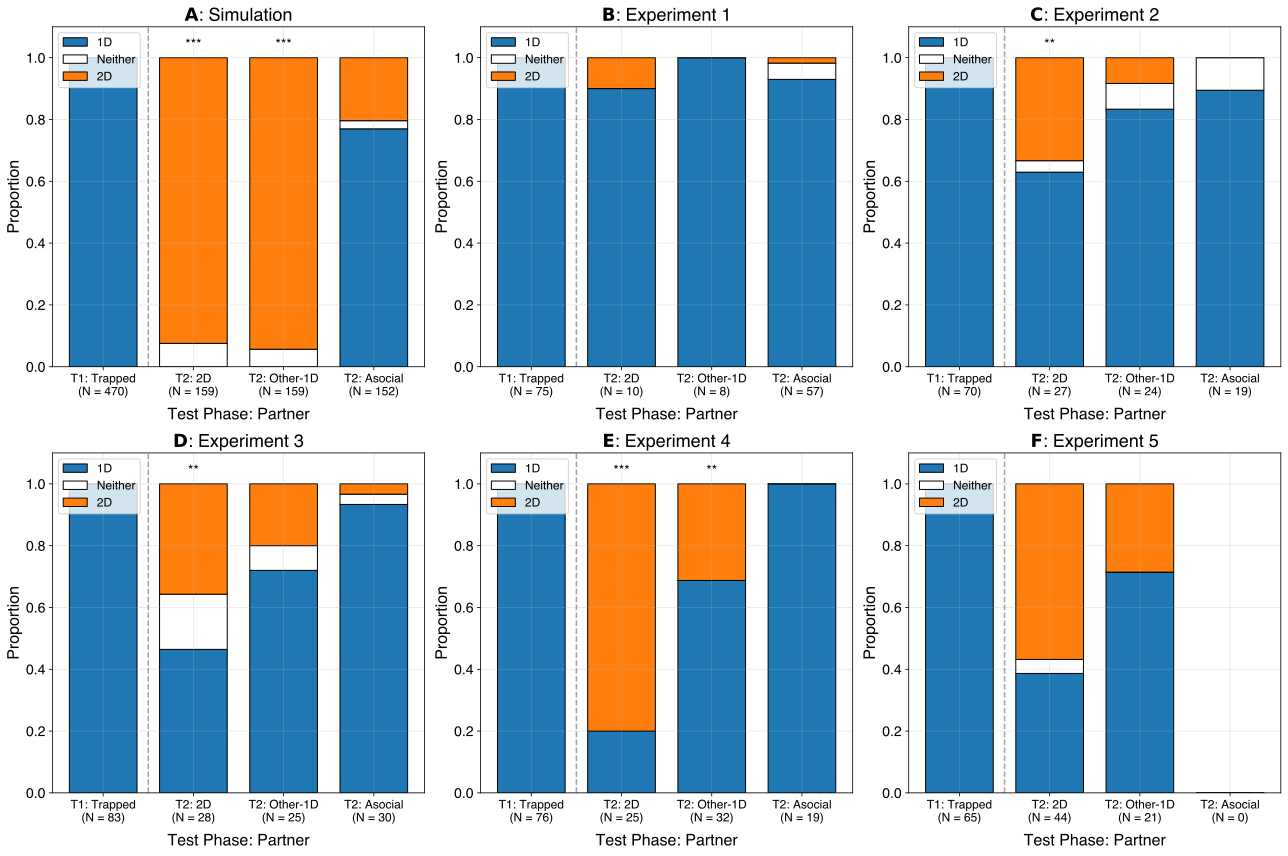
\includegraphics[width=1.0\linewidth]{trapped_learner_comparison.pdf}
    \caption{\textbf{Observational learning can help trapped learners escape, but not all informative partners are equally helpful.} All participants included in this analysis were trapped by a 1D rule in the initial test phase (T1: Trapped). The distributions to the right of the grey dashed line show the decision rule distribution of trapped learners who respectively: observed a partner using the optimal 2D decision rule (T2: 2D), a partner using the other 1D rule (T2: Other-1D), and who did not observe a partner (T2: Asocial). Participants with an optimal 2D partner were significantly more likely to escape their traps compared to asocial controls, while those observing alternative 1D strategies showed weaker benefits. Asterisks indicate significant differences in the 2D proportion from asocial controls (***: $p < 0.001$, **: $p < 0.01$, *: $p < 0.05$). (A) Selective value shaping simulation predicts that observational learning would help the vast majority of trapped learners learn the optimal 2D rule. Moreover, it predicts that 2D and other-1D partners would be equally helpful to trapped learners. (B-C) The first two experiments demonstrate that while observing a 2D partner can help trapped learners, the effect is much more modest than the simulation predictions. Contrary to simulation predictions, 2D partners are more helpful than other-1D partners. (D) There was a limited positive effect of knowing an informative partner's score in helping trapped learners to learn from them. (E) There was a large positive effect of knowing an informative partner's decision rule in helping trapped learners to learn from them, indicating that social decision rule inference was a limiting factor in observational learning (F) Adding a partner choice prediction phase prior to the observational learning phase also helped trapped learners better learn from informative partners. There are no significance markers here as we did not collect asocial control data in this experiment).}
    \label{fig:trapped-second-test}
\end{figure}
%TC:endignore

\section{Experiment 1}

Experiment 1 was our first attempt at exploring the influence of observational learning on the learning trap phenomenon.  Human participants were paired over the Internet with other humans who performed the same learning task.  In the observational learning stage of the task, participants could see each other's choices and we measured the effect it had on the prevalence and maintenance of learning traps.

\subsection{Method}

\subsection{Transparency and openness}
Data and statistical analsysis code are publicly available at \url{https://github.com/rhezab/social-escape-from-learning-traps}. The study materials and experiment code are publicly available at \url{https://github.com/rhezab/dyadic-learning-trap-task}. The following procedure was approved by the NYU Institutional Review Board (IRB-FY2023-6895). Data collection and storage were consistent with the guidelines enforced by the NYU IRB. 

\subsubsection{Participants} 

We recruited participants from the online recruitment platform Prolific (\url{https://www.prolific.com/}), restricting our recruitment to participants who: were current residents of the USA, were fluent English speakers, had an average approval rating of at least 95, and had completed at least 50 submissions. For our recruitment, we disabled the ``naivety distribution" feature from Prolific recruitment, which normally limits the rate of participant recruitment. This was done so that we could recruit enough participants in a short enough time window to match them with other participants. 

Our final sample consisted of 220 participants, of which 103 were placed in the social observational learning condition and 117 were placed in the asocial control condition. This sample size was chosen such that there were approximately 100 participants in both conditions (social and asocial), which was the approximate sample size in \citeauthor{richLimitsLearningExploration2018} \citeyear{richLimitsLearningExploration2018}. 

Seven participants were excluded for using external aid (such as using pen and paper to remember stimuli-reward contingencies), and eight participants were excluded from the social condition for having partners with missing data (i.e., we failed to successfully save their data). We did not exclude participants if their partner used external aid, which is why there are odd numbers of participants in each condition. Overall, the 220 participants came from 123 dyads (not all dyads were completely represented in the final list of participants). There were 54 dyads from the social condition, and 69 dyads from the asocial control condition. Participants received \$11.25 for participation (45 minutes at a rate of \$15 per hour) and received a performance-based bonus that ranged up to \$4.


\subsubsection{Design and Procedure}

 The task was presented as a webpage written in Javascript.  
As described above, participants completed an approach-or-avoid decision-making task with cartoon bees varying along four binary feature dimensions.  Approaching a friendly bee earned one point, while approaching a dangerous bee resulted in a five-point loss. Avoiding any bee yielded zero points and provided no information about the bee's friendliness. Participants began with 20 points and aimed to optimize their final point total for a cash bonus.  Unknown to participants, only two of the four visible features perfectly predicted whether bees were friendly or dangerous. The optimal decision strategy required attending to both relevant features (a 2D rule), where only bees with both ``bad" feature values were dangerous.

\textbf{Participant pairing.} Once recruited, participants were placed into a waiting room. Participants waited for a maximum of 10 minutes to be paired with another participant. If we were unable to pair a participant after 10 minutes, they were disconnected from the waiting room and compensated for their time waiting. Participant pairing and subsequent synchronization was implemented using Firebase Realtime Database, which allows for real-time data synchronization across multiple web browser clients. If a participant's partner left partway through the task, the remaining participant was partially compensated proportional to the time they spent on the task. 

The experiment investigated whether observational social learning could help participants escape these learning traps. Participants were paired with another participant and completed the following phases.



\textbf{Individual learning.} First, participants underwent an individual learning phase consisting of 4 blocks of 16 trials each, with each block containing the complete stimulus set. Each half-block of 8 trials contained 6 friendly bees and 2 dangerous bees to maintain consistent exposure to bee types. On each trial, participants saw a cartoon bee in the center of the screen. Within 10 seconds, they must decide whether to approach or avoid it. If they did not make a choice within 10 seconds, the trial resumed as if they had decided to avoid the bee (and we recorded that they did not make a valid choice). They made their choice either by pressing the associated keys (``F'' and ``J'' respectively) or by clicking on the corresponding buttons. Their choice was then shown on screen for 2 seconds, and the outcome of their choice was shown for 3 seconds. On the outcome screens, participants also saw the points they earned on the trial, their total score, and the number of hives remaining in the phase. Each dyad was synchronized such that they started each trial together.

\textbf{Initial test phase.} After individual learning, participants completed a test phase without feedback that comprised 2 blocks of trials to assess their decision strategy. In the test phase, participants were allowed 20 seconds to make their choice (instead of 10 seconds as in the learning phase). Their choice was then shown for 2 seconds, as before, but the outcome was not shown and they immediately progressed onto the next trial. 

\textbf{Second learning phase (social or asocial).} Participants then proceeded to a second learning phase, assigned to either a social learning condition or an asocial control condition. In the social condition, participants continued the task while observing their partner's choices. In the asocial control condition, participants completed another individual learning phase identical in structure to the first. This second learning phase also consisted of 4 blocks of 16 trials. Participants in both conditions were paired with partners and waited to start each trial together, and were not informed beforehand which condition they would experience.

Like in the individual learning phase, each trial of an observational learning phase started with the participant being presented with a cartoon bee and having to make a choice within 10 seconds. Next, they saw their own choice -- as before -- but now with their partner's choice displayed above it (for 2 seconds). Finally, each trial ended as before: they saw their outcome for 3 seconds. 

\textbf{Final test phase.} Following the second learning phase, participants completed a final test phase of 2 blocks without feedback. Strategy changes between test phases were analyzed to determine whether observational learning reduced the prevalence of learning traps compared to additional individual learning.


\subsection{Results}

In each test phase, we classified participants' behavior as following either the optimal 2D decision rule, a sub-optimal 1D decision rule (a learning trap), or neither. Following Rich and Gureckis (2018), a participant was classified as following a decision rule if 30/32 choices during the test phase were consistent with the decision rule (1D or 2D), otherwise the participant was assigned to the ``neither" category. % There are 16 unique bees, each shown twice during the test phase, so this criterion allows for two deviations from the rule over two full passes of the stimulus set. 

We first confirmed that learning traps emerged as expected, replicating \citeauthor{richLimitsLearningExploration2018} \citeyear{richLimitsLearningExploration2018}. In the first test phase, 47\% of participants employed a 1D decision rule ($N=220$; Fig.~\ref{fig:first-test}). Importantly, these 1D rules were genuine learning traps: in the asocial control condition, 93\% of trapped learners remained trapped after additional individual learning, with only 2\% learning the optimal 2D rule ($N=57$; Fig.~\ref{fig:trapped-second-test}B).

Contrary to our prediction, trapped learners in the social observational learning condition did not fare any better than trapped learners in asocial control condition. Only 2\% of trapped learners in the social condition learned the optimal 2D rule ($N = 47$), showing no significant improvement over asocial controls ($P = 1.0$).\footnote{All significance tests are two-sided permutation tests with 10,000 permutations.}) The vast majority (94\%) remained trapped in the same 1D rule. 

The lack of effect of observational social learning was partly due to the rarity of informative partnerships for trapped learners -- i.e., trapped learners were rarely paired with partners who followed either the optimal 2D rule or the other 1D rule (who would approach the bee that the trapped learner is mistakenly avoiding). Only 18 trapped learners of 47 in the social condition were paired with an informative partner. Of these, 10 trapped learners were paired with someone following the optimal 2D rule, and 8 were paired with someone following the other 1D rule. However, even when paired with an informative partner, almost all trapped learners remained trapped. Of the 10 trapped learners paired with a 2D partner, only one ended up learning the optimal 2D rule (Fig.~\ref{fig:trapped-second-test}B) -- a proportion not significantly different than in the asocial control condition ($P=0.28$, $N_{\text{social}} = 10$, $N_{\text{asocial}} = 57$). We verified that these 2D partners were reliable demonstrators of the optimal 2D rule. Out of the 10 2D partners, 8/10 employed the optimal 2D decision rule in all four observational learning phases, and the remaining 2 employed the optimal 2D rule in all but the first observational learning phase. This rules out the possibility that trapped learners failed to learn their partner's 2D rule because their partners strayed from the 2D rule during the observational learning phase.

\subsection{Discussion}

Contrary to the prediction of our value-shaping simulation, we found that the prevalence of trapped learners was not reduced by observational social learning. This was partly due to the rarity of informative partnerships, but also reflected trapped learners' apparent inability to learn from informative partnerships. Given the small sample size of informative partnerships, however, we could not definitively say that trapped learners were unable to learn from informative partners. Given this, in Experiment 2 we further investigated the question of whether trapped learners can learn from informative partnerships by exerting additional experimental control.



\section{Experiment 2}

In Experiment 1, we found that trapped learners were mostly unable to learn from informative partnerships (i.e., those where the partner approached items that the current participant did not). However, this finding was based on a small number of informative partnerships (only 18 in total) that emerged within human dyads. In Experiment 2, we again investigated whether trapped learners could learn from informative partnerships, however, instead of pairing people with other humans, we paired participants with simulated partners that follow programmed decision rules. This allowed us to make sure that trapped learners would observe informative choices during the observational learning phase. Simulated partners followed either the optimal 2D rule or one of two sub-optimal 1D rules. 


\subsection{Participants}

Our final sample consisted of 184 participants, of which 140 were placed in the social observational learning condition and 44 were placed in the asocial control condition (and an equal number of human-bot dyads in each). We aimed for a sample of approximately 45 participants in each of the following conditions: asocial condition, social condition with 2D partner, social condition with other-1D partner, social condition with same-1D partner. This aim was based on the expectation that this would result in approximately 20 trapped learners in each of the above conditions, since we expected about half of all learners to get trapped after individual learning (based on the results of Experiment 1). Participants were initially randomly assigned to each of the four conditions, but later there was targeted assignment to fulfill recruitment goals. Four participants were excluded for using external aid (e.g., using pen and paper). Participants were recruited from Prolific and received \$10 for participation (40 minutes at a rate of \$15 per hour) and received a performance-based bonus that ranged up to \$4.


\subsection{Design and Procedure}

The experiment followed the same logic and design as Experiment 1 with two key changes. First, participants were paired to simulated partners with programmed decision rules instead of other real human participants. Participants were told that they would either be matched with a real human participant or a simulated partner. As in Experiment 1, they entered a waiting room where we simulated a waiting time of 7.3 seconds. Partner choice times were simulated using a Gamma distribution with a shape parameter ($\alpha$) of 2.69, a scale parameter ($\theta$) of 0.55, and a location parameter ($\gamma$) of 0.0055. These parameters were chosen such that the distribution of simulated choice times roughly matched the distribution of participant choice times from Experiment 1. 


Second, we changed the graphic design of the choice and outcome feedback screens in Experiment 2. The choice screen now showed an animated avatar (representing the participant) approaching or avoiding the bee. In an observational learning phase, the choice screen also showed another animated avatar (representing the simulated partner) approaching or avoiding the bee. The outcome screen now showed either a drop of honey or a stinger emerging from the bee. Due to a coding error in the new outcome screens, participants were shown their total score in the test trials. This meant that participants could have inferred the outcomes of their choices during test trials by noting changes in their total score, even though the choice outcomes were not explicitly shown during test trials.  Our results suggest that this small error had little overall effect and it was corrected in subsequent experiments.


All other aspects of the experiment were identical to Experiment 1.

\subsection{Results}

As in Experiment 1 and in \citeauthor{richLimitsLearningExploration2018} \citeyear{richLimitsLearningExploration2018}, we found that sub-optimal 1D decision rules were prevalent in the first test phase before observational learning. Forty-eight percent of participants employed a 1D rule in the first test phase (\ref{fig:first-test}, $N=184$). As before, we empirically verified that these 1D decision rules were indeed learning traps. In the asocial control condition, 89\% of trapped learners remained trapped after an additional individual learning phase (\ref{fig:trapped-second-test}C, $N=19$). Moreover, none of them learned the optimal 2D rule during the second individual learning phase ($N=19$). This shows that learners that followed a 1D rule by the first test phase were truly trapped (despite the possibility of inferring choice outcome feedback during the first test phase due to the coding error). 

In contrast, some ``trapped learners" in the social condition were able to learn the 2D rule during the observational learning phase. After observing the optimal 2D rule, a third of trapped learners were able to learn the optimal 2D rule by the second test phase -- a statistically significant increase compared to the asocial control condition (Fig.~\ref{fig:trapped-second-test}C; $P<0.01$, $N_{\text{social}}=27$, $N_{\text{asocial}}=19$). When observing the other 1D rule, however, only 8\% of trapped learners were able to learn the optimal 2D rule. This was not a statistically significant improvement over the asocial control condition (Fig.~\ref{fig:trapped-second-test}C; $P=0.49$, $N_{\text{social}}=24$, $N_{\text{asocial}}=19$). 

As predicted, trapped learners that learned the 2D rule via observational learning were able to do so without costly extended exploration: 8 out of 11 who learned the 2D rule did so without approaching any dangerous bees during the observational learning phase (Fig.~\ref{fig:trapped-to-optimal-heatmaps}C). Rather than broad exploration, those that learned the 2D rule during the observational learning phase seemed to do so by inferring the rule guiding their partner's approach/avoid choices and selectively exploring in a manner guided by their partner's rule.  

%TC:ignore
\begin{figure}
    \centering
    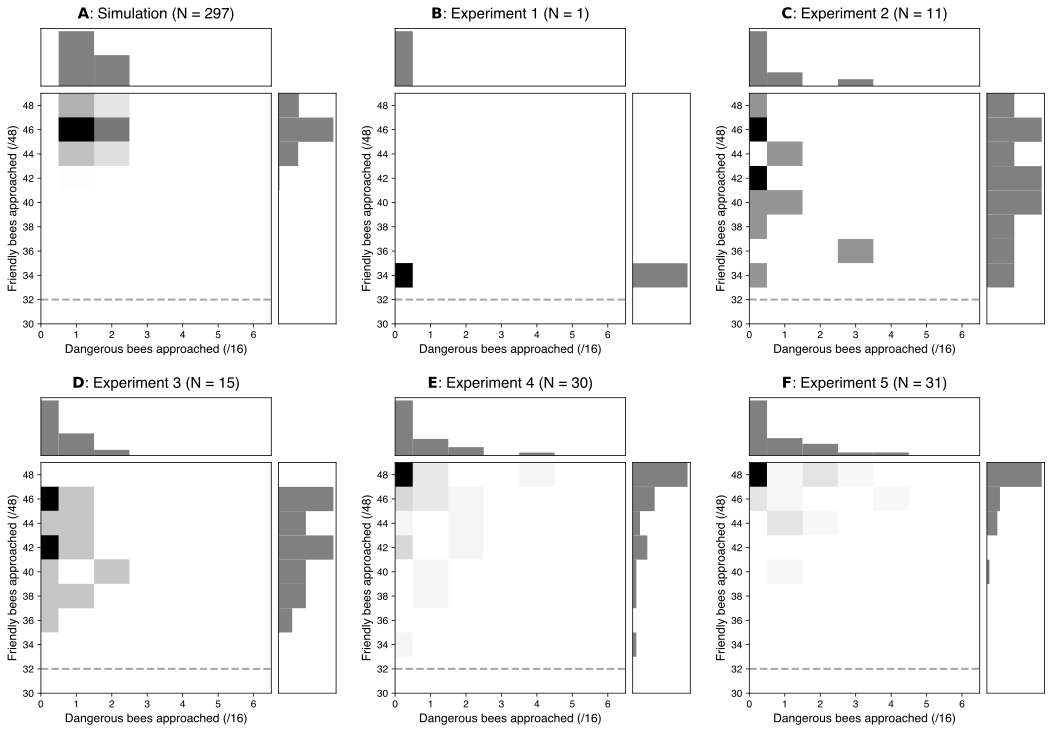
\includegraphics[width=1.0 \linewidth]{trapped_to_optimal_grid.pdf}
    \caption{\textbf{Trapped learners escape through observational learning without costly exploration.} Heatmaps showing friendly versus dangerous bees approached during the observational learning phase for participants who successfully learned the optimal 2D rule. Each panel displays the exploration patterns of trapped learners who escaped their learning traps by observing partners. Most participants learned the optimal strategy without approaching any dangerous bees (shown by concentration along the left side edge), avoiding the typical costs of individual exploration.}
    \label{fig:trapped-to-optimal-heatmaps}
\end{figure}
%TC:endignore

\subsection{Discussion}

The results of Experiment 2 were partially consistent with the qualitative predictions of our selective value-shaping simulation. Our first prediction was that trapped learners would be significantly more likely to escape their trap and learn the 2D rule in the observational learning condition compared to the asocial control condition. We did find that a significant proportion of trapped learners were able to escape the learning trap after observing an optimal 2D partner. However, the majority of them remained trapped. Moreover, a smaller and insignificant proportion of participants were able to escape the learning trap after observing an other-1D partner. This disagreed with our second prediction: that observing either the optimal 2D rule or the other 1D rule would be similarly beneficial for trapped learners. Finally, in agreement with our third prediction, we did find that trapped learners who learned the 2D rule were able to do so without costly extended exploration. 

With these results in mind, we turned our attention to the following question: what was stopping most trapped learners from learning the 2D rule via observational learning? We hypothesized that there were two main limiting factors: i) they did not trust that their partners were making good choices, or (ii) they were unable to infer the decision rule guiding their partner's choice to approach bees that they were avoiding. Either factor could cause a trapped learner to fail to learn the 2D rule despite the necessary information. We explore these factors in the next experiments. 

\section{Experiment 3}
In Experiment 3, we investigated the hypothesis that trapped learners did not benefit from observational learning in Experiments 1 \& 2 because they did not trust that their partners were making good choices. That is, they ``explained away" their partner's choices as errors, falsely believing that they had nothing to learn from the choices they were observing. We also asked whether such ``explaining away" might also account for the discrepancy between how likely trapped learners were to learn from observing the optimal 2D decision rule versus observing the other 1D rule, even though both rules provide the evidence necessary to escape the learning trap. 

\subsection{Task} 

Experiment 3 was identical to Experiment 2, except that participants in the social condition were told their partner's score from the first test phase before the observational learning phase commenced. They were also shown their own score for comparison. We reasoned that if trapped learners failed to engage in observational learning because they falsely believed that they had nothing to learn from their partner, then showing them their partner's decision rule would provide the necessary signal that their partner's choices are informative. When paired with someone following the optimal 2D rule, the trapped learner would see that their partner performed better than them. When paired with someone following the other 1D rule, the trapped learner would see that it was possible to achieve approximately equivalent performance by attending to a different feature -- signaling the relevance of that feature, which was previously ignored by the trapped learner. 

We also corrected the error on the outcome screen from Experiment 2 so that the total score was correctly omitted during test trials.

\subsection{Participants} 

Our final sample consisted of 199 participants, of which 105 were placed in the social observational learning condition and 94 were placed in the asocial control condition. We aimed for a sample of approximately 45 participants in each of the following conditions: asocial condition, social condition with 2D partner, and social condition with other-1D partner. This aim was based on the expectation that this would result in approximately 20 trapped learners in each of the above conditions, since we expected about half of all learners to get trapped after individual learning (based on the results of Experiment 1). All participants were randomly assigned. We ended up collecting double the amount of participants in the asocial control condition due to an error in the random assignment logic. Four participants were excluded for using external aid. Participants were recruited from Prolific and received \$7.50 for participation (30 minutes at a rate of \$15 per hour) and received a performance-based bonus that ranged up to \$4.

\subsection{Results} 

After observing the optimal 2D decision rule, 36\% learned the optimal decision rule (Fig.~\ref{fig:trapped-second-test}D; $P<0.005$, $N_{\text{social}}=28$, $N_{\text{asocial}}=30$), compared to 33\% in Experiment 2. After observing the other 1D rule, 20\% of trapped learners were able to learn the optimal 2D rule (Fig.~\ref{fig:trapped-second-test}D; $P=0.09$, $N_{\text{social}}=25$, $N_{\text{asocial}}=30$), compared to 8\% in Experiment 3. In both cases, there was no significant difference between Experiments 2 and 3 ($P=1.0$ and $P=0.41$ respectively), though the latter is suggestive of an effect that might become significant with a larger sample size. 

\subsection{Discussion}

Overall, we did not find evidence that telling trapped learners their partner's score made them much more likely to learn from their partner. This finding suggests that trust in partners' competence is not a key limiting factor for observational learning in our task. It also suggests that seeing others achieve higher scores was not enough to encourage trapped learners to engage in broad individual exploration, despite previous studies showing the effectiveness of showing trapped learners the gap between current rewards and optimal earnings as an intervention \cite{leeOvercomingLearningTraps2023}. 

\section{Experiment 4}
In Experiment 4, we tested the hypothesis that most trapped learners did not benefit from observational learning in Experiments 2 \& 3 because they failed to infer the decision rule that generated their partner's choices. 

\subsection{Task} 
Experiment 4 was identical to Experiment 2, except that before the observational learning phase, participants were asked to answer the question ``Which bees should you avoid?" (to increase the credibility of the manipulation) and in the social condition subsequently viewed a generated "response" from their (bot) partner. An example description of a 2D decision rule reads: ``Avoid bees with both antennae and dots on their body." Experiment 4 is identical to Experiment 2 in all other ways. We reasoned that if trapped learners did not benefit from observational learning because they had failed to infer their partner's decision rule, then more trapped learners would benefit from observational learning in Experiment 4. 

\subsection{Participants} 

Our final sample consisted of 192 participants, of which 139 were placed in the social observational learning condition and 53 were placed in the asocial control condition. We aimed for a sample of approximately 50 participants in each of the following conditions: asocial condition, social condition with 2D partner, and social condition with other-1D partner. This aim was based on the expectation that this would result in at least 20 trapped learners in each of the above conditions, since we expected about half of all learners to get trapped after individual learning (based on the results of Experiment 1). All participants were randomly assigned. Seven participants were excluded for using external aid. Participants were recruited from Prolific and received \$7.50 for participation (30 minutes at a rate of \$15 per hour) and received a performance-based bonus that ranged up to \$4.

\subsection{Results} 

After being told another person's 2D rule and observing choices made according to it, 80\% of trapped learners were able to adopt the optimal 2D rule (Fig.~\ref{fig:trapped-second-test}E; $P<1/10,000$, $N_{\text{social}}=25$, $N_{\text{asocial}}=19$). For comparison, in Experiment 2, only a third of trapped learners observing a 2D rule were able to learn the 2D rule themselves (Fig.~\ref{fig:trapped-second-test}C; $P<0.001$, $N=27$). After observing the other 1D rule, 31\% of trapped learners were able to learn the optimal 2D decision rule (Fig.~\ref{fig:trapped-second-test}E; $P<0.01$,  $N_{\text{social}}=32$, $N_{\text{asocial}}=19$). For comparison, in Experiment 2, only about 8\% of trapped learners observing the other 1D rule were able to learn the optimal 2D rule (Fig.~\ref{fig:trapped-second-test}C; $P=0.051$, $N=24$). As before, trapped learners in Experiment 4 were more likely to learn from the optimal 2D rule versus the other 1D rule. 

\subsection{Discussion}

In this experiment, we found that telling participants their partner's decision rule -- so that they don't have to infer it -- made trapped learners more likely to escape their trap via observational learning. This finding suggests that social decision rule inference is a major limiting factor for observational learning in our task, and that allowing explicit natural language communication between individuals can significantly boost the effectiveness of social interventions for learning traps.

Moreover, this finding further suggests that trust in partner competence is not a major limiting factor for observational learning when observing a partner employing the optimal 2D rule -- once a participant knows their partner's 2D rule, the overwhelming majority of them decide to employ their partner's 2D rule (Fig.~\ref{fig:trapped-second-test}F). Notably, the majority of trapped learners observing an other-1D partner remained trapped. This suggests that integrating the other 1D rule with one's own remains challenging, with trust in partner competence potentially playing a role. This result is theoretically notable, since our selective value-shaping model does not account for such a difference in observational learning success between observing a 2D partner or other-1D partner. Moreover, the selective value-shaping model also does not account for social decision rule inference as a limiting factor, since in that model observing others' choices directly influences choice values, without an intermediate social decision rule inference step. 

\section{Experiment 5}

%TC:ignore
\begin{figure}
    \centering
    \includegraphics[width=0.9 \linewidth]{partner_prediction_combined_figure.pdf}
    \caption{\textbf{Social decision rule inference success determines observational learning success.} (A) In Experiment 5, less than half of trapped learners successfully inferred an informative partner's decision rule. Participants who made one or fewer mistakes in predicting their partner's choices in the final partner choice prediction block were judged to have successfully inferred their partner's decision rule. (B) Trapped learners who successfully (S) inferred an informative partner's decision rule were more likely to subsequently adopt the optimal 2D decision rule in the second test phase. Asterisks indicate significant differences in the 2D proportion between trapped learners who either succeeded (S) or failed (F) to infer an informative partner's decision rule (***: $p < 0.001$)} % , **: $p < 0.01$, *: $p < 0.05$).}
    \label{fig:partner-prediction}
\end{figure}
%TC:endignore

After Experiment 4, it remains unclear whether decision inference is prohibitively challenging in our task or whether rule inference success can be improved either by directly incentivizing it or by allowing participants to observe their partner's choices without having to make their own choices on the same trial, enabling them to allocate more cognitive resources towards inferring their partner's decision rule. We sought to answer this question in Experiment 5. We also sought to collect explicit measures of participants' ability to infer their partner's decision rule, so that we could directly test the hypothesis that successful social decision rule inference is predictive of learning trap escape via observational learning.

\subsection{Task}

In Experiment 5, we introduced a partner prediction phase that preceded the observational learning phase. Like each learning phase, the partner prediction phase consisted of 4 blocks of 16 trials each (showing each of the 16 unique bees once). Each trial of the partner prediction phase proceeded as follows. First, the bee stimulus was shown and the participant were asked to predict their partner's choices (``Approach" or ``Avoid"). Then, their partner's choice was shown along with prediction feedback. Participants were awarded +1 point for each correct prediction and no points for an incorrect prediction. Note that participants did not make their own choices during the partner prediction phase, nor were they rewarded or punished for the outcomes of their partner's choices. There was no asocial control condition in Experiment 5, as we were primarily interested in comparing the observational learning outcomes of participants who successfully inferred their partner's decision rule to participants who failed to infer their partner's decision rule. Moreover, we believe that the asocial control condition in previous experiments firmly established the lack of learning without a social component. Experiment 5 is identical to Experiment 2 in all other respects. 

\subsection{Participants}

Our final sample consisted of 192 participants, all of whom took part in the ``partner prediction'' phase. We aimed for a sample of approximately 70 participants in each of the following conditions: social condition with 2D partner, and social condition with other-1D partner. This aim was based on the expectation that this would result in approximately 30 trapped learners in each of the above conditions, since we expected about half of all learners to get trapped after individual learning (based on the results of Experiment 1). All participants were randomly assigned. We ended up collecting double the amount of participants in the social with 2D partner condition due to an error in the random assignment logic. Five participants were excluded for using external aid. Participants were recruited from Prolific and received \$10 for participation (40 minutes at a rate of \$15 per hour) and received a performance-based bonus that ranged up to \$4.

\subsection{Results}

Overall, the partner prediction phase seemed to help more trapped learners escape their learning trap via observational learning: 57\% of trapped learners who observed the optimal 2D decision rule were able to learn it (Fig.~\ref{fig:trapped-second-test}F; $N=44$) while 29\% of trapped learners who observed the other 1D decision rule were able to learn it (Fig.~\ref{fig:trapped-second-test}F; $N=21$). Compared to Experiment 2, more trapped learners were able to learn the 2D rule after observing either the 2D rule or the other-1D rule, though this difference was not statistically significant given our small sample size ($p=0.085$ and $p=0.12$ respectively).

We did find that participants who successfully inferred their partner's decision rule were significantly more likely to adopt a 2D partner's rule. To assess whether participants successfully inferred their partner's decision rule, we used a strict criterion: participants needed to make at most one error when predicting their partner's choices in the final prediction block. Using this criterion, we found that less than half (44\%) of trapped learners with informative partners successfully inferred their partner's decision rule (Fig.~\ref{fig:partner-prediction}A; $N=65$). The relationship between rule inference and learning was particularly striking for participants who observed the optimal 2D rule. Among those who successfully inferred the 2D rule, nearly all (95\%) went on to adopt it themselves ($N=19$). In stark contrast, of those who failed to infer the 2D rule, almost none (4\%) managed to learn it (Fig.~\ref{fig:partner-prediction}B; $N=25$, $P<1/10,000$). We found a similar pattern, though less pronounced, among participants who observed the alternative 1D rule. Half of the participants who successfully inferred the 1D rule eventually learned the optimal 2D rule ($N=10$). Among those who failed to infer the 1D rule, only 10\% learned the 2D rule, though this difference was not statistically significant given our small sample size (Fig.~\ref{fig:partner-prediction}B; $N=10$, $P=0.07$). Finally, it is notable that trapped learners who escaped their trap were able to approach all friendly bees while avoiding all dangerous bees during the observational learning phase (Fig.~\ref{fig:trapped-to-optimal-heatmaps}F).

\subsection{Discussion}

The results of Experiment 5 provide direct evidence linking social decision rule inference to social escape from learning traps -- when a trapped learner inferred a 2D partner's decision rule, they went on to adopt the optimal 2D rule. Moreover, although the comparison to Experiment 2 was not statistically significant, the results of Experiment 5 also suggested that an intervention which encourages participants to learn their partner's decision rule -- such as the partner prediction phase -- can help trapped learners escape their learning trap. Directly incentivizing participants to infer their partner's decision rule may have helped, although there are known limits to the incentivization of cognitive discovery \cite{osbornpoppCanCognitiveDiscovery2025}. 

\section{General Discussion}

Individual learners often show a tendency to engage in self-reinforcing avoidance, a pattern referred to as a learning trap~\cite{denrellAdaptationInformationRestriction2001, richLimitsLearningExploration2018}.  However, most of our learning occurs in social settings where we might benefit from the exploration and information of others.  In the present report, we investigated the hypothesis that observational social learning might help learners escape the loop of self-reinforcing avoidance~\cite{allidinaAvoidanceBegetsAvoidance2021,hayesOvercomingLearningTraps2025}. Replicating prior work we found that individual learning traps were pervasive~\cite<c.f.,>{richLimitsLearningExploration2018, liCanLossesHelp2021}, but we additionally found that the majority of trapped learners remained trapped despite observational learning opportunities (Experiments 1-2). 
%This result is consistent with a recent study reporting limited benefits of observational learning~\cite{hayesOvercomingLearningTraps2025}. 
Our subsequent experiments sought to elucidate the factors why observational learning was ineffective at helping people escape these traps.

We first hypothesized that allowing participants to see their partner's score prior to observational learning would encourage trapped learners to trust the competence of their partner. Instead, we found that this information had little effect (Experiment 3), suggesting that trust in partners' competence was not a major limiting factor in earlier experiments. Next, we hypothesized that allowing participants to read a natural language description of their partner's decision rule would help trapped learners who might have otherwise failed to infer their partner's decision rule. This information had a large effect, with 80\% of trapped learners successfully adopting the optimal 2D rule after observing a partner demonstrate it (Experiment 4). This dramatic improvement suggests that the difficulty of inferring another person's decision rule was a major limiting factor in earlier experiments. Experiment 5 provided further evidence for this conclusion. In a variant of the observational learning task in which social decision rule inference was explicitly encouraged and cognitive load was reduced by eliminating concurrent choice,  trapped learners' ability to predict their partner's choices -- a measure of their successful social decision rule inference -- also predicted their escape from a learning trap. Collectively, these studies suggest that social observational learning can help individuals escape from learning traps, provided the decision rule of an observed partner can be readily inferred. 

Several properties of our task made social decision rule inference important. Participants could not communicate with their partners (with the exception of Experiment 4), but instead had to learn solely from observing their partner's choices. Moreover, as approaching a dangerous bee incurred a large loss of points, individual exploration was costly, discouraging broad exploration to discover the motivation for a partner's divergent choices. Because participants had to make their own choice before seeing their partner's choice on any given trial, they could not simply copy a partner's choices (to copy they would need to remember a partner's previous choice from many trials ago). Finally, as participants had to learn about 16 unique stimuli with 4 binary features, they could not feasibly memorize their partner's choice for each unique stimulus due to working memory constraints. Inferring a partner's decision policy, and then explicitly comparing it to one's own strategy, may be a faster and more effective way to detect and repair errors in decision making. In general, social decision rule inference may be necessary for social learning in situations that afford limited communication, costly exploration, inability to copy, and involve complex stimuli or states, where the decision-relevant features may not be apparent. 

In our experiments, we had to ``help" people infer the policy of their partner.  This is likely because social decision rule inference, even in this simple task, was difficult. Learners faced a vast hypothesis space of possible decision rules, with 16 possible combinations of relevant features and many possible decision rules for each possible combination (e.g., ``avoid if bee has antennae and dots", ``avoid if bee has antennae or dots", ``avoid if bee has antennae or dots", etc.). Previous work has shown that people struggle to learn complex multi-feature concepts solely from examples without any linguistic guidance~\cite{sumersShowTellExploring2023}. More generally, the complexity of a concept or algorithm has a negative effect on its transmissibility \cite{thompsonComplexCognitiveAlgorithms2022a}. Another consideration which may have made social decision rule inference in our task particularly challenging is that participants must generate and test hypotheses ``online", since they can only view one trial at a time. They also had to make their own choices, adding to the working memory load. In general, we expect social decision rule inference to be difficult when there are many potentially relevant features and many possible rules over those features. Of course, the challenge of searching large hypotheses spaces also applies to individual learning, which may help explain why so many learners in our task initially get trapped by simple 1D rules. 

At the beginning of our study, we hypothesized that participants would behave in accordance with the selective value-shaping mechanism we had initially proposed. These predictions were partially correct. The selective value-shaping simulations correctly predicted that trapped learners could escape by observing a 2D partner, and that they would do so largely via vicarious learning, rather than through individual exploration. However, the selective-value shaping simulations did not predict the relative inefficacy of observing a 1D partner using a different decision rule. The model also did not predict the overall persistence of the learning trap -- even after observing a partner demonstrating the optimal 2D rule, the majority of participants remained trapped (Experiments 1-2). 

Given the apparent importance of social decision rule inference in this task, an explicit rule inference model~\cite{goodmanRationalAnalysisRuleBased2008, chandraTheoriesMindLanguages2025} seems like a natural alternative to the selective value-shaping model we initially proposed. With appropriate design choices, such a model may account for both the successes and failures of observational learning in our task. For example, we could possibly account for variance in social decision rule inference success by introducing recency-biased stochastic sampling of observations for hypothesis generation and testing (reflecting working memory limitations). Indeed, modeling working memory constraints has been shown to help account for variance in human behavior \cite{collinsHowMuchReinforcement2012}. An important topic for future research is the mechanisms underlying how trapped learners integrate individual experience and social observations 
\cite{dalegeFormalizedAccountAttitudes2016, mollemanStrategiesIntegratingDisparate2020, wittHumansFlexiblyIntegrate2024, huCommonSenseReasoning2024, suIntegrationLanguageExperience2025, colasLanguageExperienceComputational2025}. We suspect that applying an explicit rule inference model may also be fruitful here. In particular, it may help explain why trapped learners were consistently more likely to learn from a 2D partner than an other-1D partner. More concretely, when observing a 2D partner, the 2D rule can readily explain the learner's individual experiences, while when observing an other-1D partner, the learner must generate the 2D rule as a hypothesis rule that can explain both the learner's individual experiences and their partner's other-1D rule. This requirement for hypothesis generation in the latter case may explain why successful social learning is more likely in the former case. Another possibility is that a trapped learner is less likely to learn from someone following an other-1D rule because the other-1D rule avoids rewarding stimuli that the trapped learner already knows about, thus appearing to be a less competent source. Such an effect can be captured by weighted integration of another person's decision rule depending on how well it captures social learner's existing prior knowledge. 

Our findings may help better understand why stereotypes may persist despite the ability to observe disconfirmatory evidence. Recent work has demonstrated that stereotypes can function as learning traps -- false beliefs that emerge and persist through a pattern of avoidance \cite{allidinaAvoidanceBegetsAvoidance2021, baiCostlyExplorationProduces2025}. Notably, observational learning has been suggested as a possible way to ``break out of the feedback cycle of self-perpetuating avoidance" \cite{allidinaAvoidanceBegetsAvoidance2021}. Our work shows that although observational learning can indeed help people break out of learning traps, it does not guarantee it due to the challenge of inferring others' beliefs. For example, simply observing other companies increase the diversity of their workforces may not be enough to sway a company's hiring practices. Social interventions attempting to curb the influence of stereotypes on decision making should help people understand the rationale behind others' choices rather than merely exposing them to alternative choices. Returning to our earlier example, a hiring manager hoping to influence others to hire members of under-represented groups should share details of their hiring process, rather than just their hiring statistics.

\subsection{Constraints on Generality}
Although we believe that our task captures essential components of real-world learning traps (e.g., choice contingency and multi-feature stimuli), it is still a simplified laboratory task. Learning traps in the real world likely have additional social and cultural factors contributing to their persistence that we did not study here. Moreover, though we found a positive effect of natural language communication on social learning, we considered a highly restricted and artificial form of natural language communication -- the effects of real-world natural language communication remain to be studied. Similarly, though we found a positive effect of a manipulation in which social decision rule inference was directly incentivized, real-world settings in which such an intervention would be plausible are likely rare (e.g., learning to imitate a gambler or financial trader on a market platform with a plethora of choice data). 

\subsection{Conclusion}
In summary, our findings demonstrate that while observational learning can help overcome the limits of individual learning, it is itself limited by the difficulty of inferring others' decision rules. Taken together, our findings add to the substantial literature on the robustness of learning traps. Uniquely, it challenges the notion that learning traps are \emph{just} about lack of opportunities for learning. Our results show that even when the information required for learning is available, one still needs to make sense of the information to learn from it. We show that affordances around this information can make a big difference -- natural language communication significantly boosts social learning, and reducing parallel cognitive load and incentivizing social decision rule inference seems to help too. Future work should further explore the affordances that can best support effective social learning for trapped learners.


%TC:ignore
\section{Acknowledgments}
This work was supported by NSF BCS 2021060 to TMG. We would like to thank Pam Osborn Popp for her help with the experiment code. We would like to thank the following people for thoughtful discussions of this work: members of the Hartley and Gureckis labs, attendees of the Annual Meeting of the Cognitive Science Society in 2024 and 2025, and attendees of the Cognitive Computational Neuroscience conference in 2024.

\begin{figure}
    \centering
    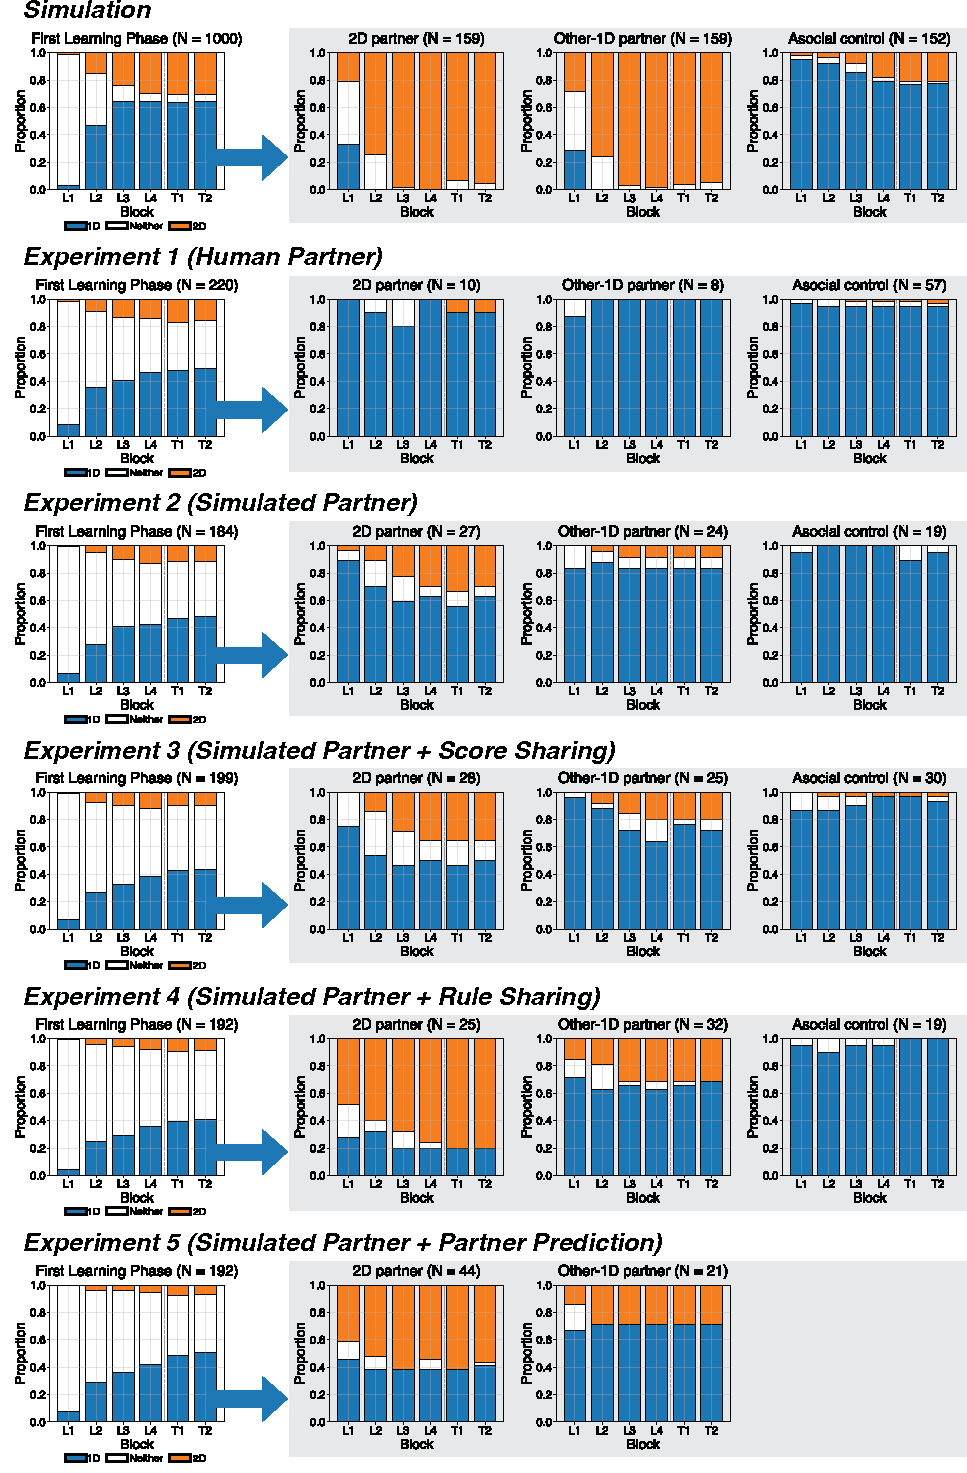
\includegraphics[width=0.8 \linewidth]{learning-phases-6.pdf}
    \caption{\textbf{(Supplementary Figure) Decision rule distributions for each learning and test block.} For each experiment, the leftmost panel shows the distributions for blocks from the first individual learning phase (for all participants). The panels within the grey box show decision rule distributions for trapped learners in each of the three named conditions during the second learning phase.}
    \label{fig:drule-distributions}
\end{figure}

\bibliographystyle{apacite}

\setlength{\bibleftmargin}{.125in}
\setlength{\bibindent}{-\bibleftmargin}

\bibliography{references}
%TC:endignore

\end{document}
